In this chapter, the performance of both the simulation model and visual SLAM method are analyzed in a series of empirical experiments.
In Section \ref{sec:simulation_results}, the USARSim simulation model is validated.
A set of maneuvers is flown with the actual AR.Drone and
simulated AR.Drone. The differences between the maneuvers are studied in detail.
In Section \ref{sec:results-position-accuracy}, the accuracy of the AR.Drone's estimated position is evaluated.
A set of 8-shapes is flown with the AR.Drone and the estimated positions are compared against the groundtruth from a laser range finder.


	\section{Simulation model}
\label{sec:simulation_results}
To evaluate the USARSim simulation model,  
a set of maneuvers is flown with the actual AR.Drone and
simulated AR.Drone. The differences between the maneuvers are studied in detail. To enable multiple repetitions of the same maneuver it is
described as a set of time points (milliseconds since initialization) each coupled to a movement command.
%We wrote wrappers for the AR.Drone programming interface and for USARSim interface which read these scripts and output a control
%signal, using the system clock to manage the timing independently from the game engine and the AR.Drone hardware.
Orientation, altitude and horizontal speed are recorded at a frequency of $200\hertz$ during the maneuvers. These are gathered through the AR.Drone's internal sensors and the onboard algorithms, which are
also used by the controller to operate the drone. The filtered output of the gyroscope is used
to estimate the orientation. The filtered output of the ultrasound distance sensor is used to estimate
the altitude. The onboard visual odometry algorithm is used to estimate the horizontal (linear
and lateral) speeds. The simulator has equivalent sensors. In addition, simulation can provide ground-truth data. 
Also for the real maneuvers an attempt was made to generate ground truth via an external reference system; the movements were recorded with a synchronized video system consisting of four firewire cameras, capturing images at 20 frames per second at a resolution of $1024 \times 768$ pixels. The position of the AR.Drone 
in each frame has been annotated by hand. 
%However, since the processing of the captured data is not yet complete, results from these trials are not presented in this paper.
%reference?!

Corresponding to NIST guidelines \cite{Jacoff2010STM}
a set of experiments of increasing complexity was performed. For the AR.Drone
four different experiments were designed.
The first experiment is a simple hover, in which the drone tries to maintain its position (both horizontal and vertical). The second experiment is linear movement, where the drone actuates a single movement command. The third experiment is a small horizontal square. The last experiment is a small vertical square.

\subsubsection{Hovering}

Quadrotors have hovering abilities just like a helicopter. The stability in maintaining a hover depends
on environmental factors (wind, underground, aerodynamic interactions) and control software.
%In \cite{Michael2010ra} a
%horizontal positioning error of no more than $2\small{cm}$ and a vertical error of less than $0.6\small{cm}$ are reported for
%a tightly optimized stiff controller. In practice, softer controllers are used which are more robust and can
%recover from larger disturbances. In \cite{How2008} a horizontal and vertical positioning error of no more than $10\small{cm}$ are %reported. 
If no noise model is explicitly added, the USARSim model performs a perfect hover; when no control signal is given the
horizontal speeds are zero and the altitude stays exactly the same.

For the AR.Drone, this is a good zero-order model. One of the commercial features of the AR.Drone is its ease of operation. As part of this feature it
maintains a stable hover when given no other commands, which is accomplished by a visual feedback loop.
%The hover is quite robust and in impromptu
%ad-hoc tests was able to recover from major attitude disturbances up to $\sim45^o$. However, in this section we
%are concerned with the hovering behavior with minor disturbances. 
So, the hovering experiment is performed  
indoors
with an underground chosen to have enough texture for the onboard visual odometry estimation algorithm.

As experiment the AR.Drone maintains a hover for 35 seconds. This experiment was repeated 10 times,
collecting 60.000 movement samples for a total of 350 seconds. Over all samples the mean absolute error in horizontal
velocity (the Euclidean norm of the velocity vector) is $0.0422\small{m/s}$ with a sample variance of $0.0012\small{m^2/s^2}$. From
the samples we obtain the distribution of the linear and lateral velocity components. 

From the velocity logs the position of the AR.Drone during the 35-second 
flight was calculated. 
%Figure \ref{fig:scatterplot} shows a scatterplot of positions over all flights.
The mean absolute error of the horizontal position is $0.0707\small{m}$ with a sample variance of $0.0012\small{m^2}$.

\begin{comment} % to save some space
\begin{figure}[htb]
\centering
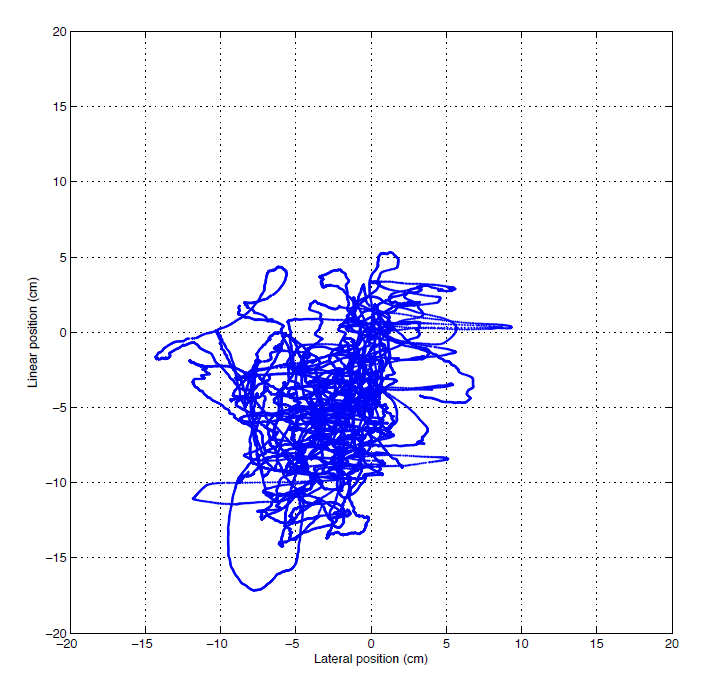
\includegraphics[width=8cm]{images/HoverScatterPlot.png}
\caption{Scatter plot of the horizontal position aggregated over all hover flights.}
\label{fig:scatterplot}
\end{figure}
\end{comment}

\subsubsection{Horizontal movement}

In this experiment the AR.Drone is flown in a straight line. It is given a control pulse (i.e., pitch) with a constant signal
for 5 different time periods: 0.1s, 1s, 2s, 3s, and 5s. Each pulse is followed by a null signal for enough time for the AR.Drone to make a full stop and a negative pulse of the same magnitude for the same period,
resulting in a back and forth movement. In Figure \ref{fig:RealResponse}
 the red line shows the control signal, the blue line the response (i.e., velocity) of the AR.Drone. The experiment was repeated for 5 different speeds.
The control signal $s$ specifies the pitch of the AR.Drone as a factor (between 0 and 1) of the maximum absolute tilt $\theta_{max}$, which was set to the default value\footnote{ARDrone firmware (1.3.3)}. % iPhone uses 12deg
The trials were performed with the
values of 0.05, 0.10, 0.15, 0.20, 0.25 for the control signal $s$.

\begin{figure}[htb]
\centering
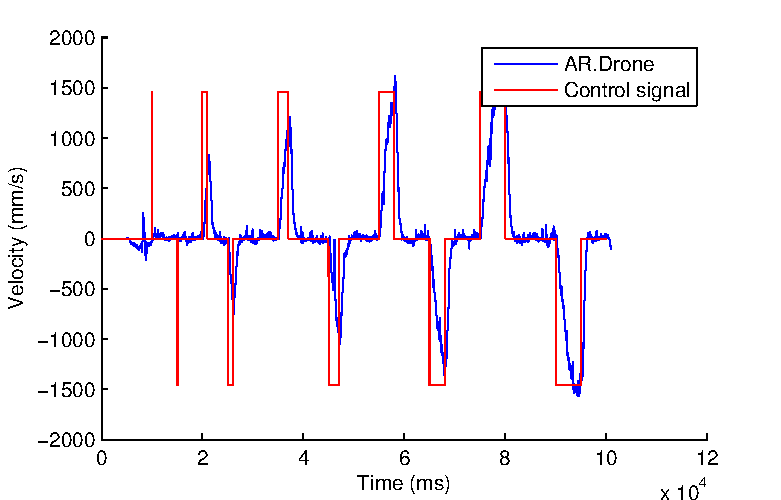
\includegraphics[width=11cm]{images/Dr7Ov-eps-converted-to.pdf}
\caption{Velocity of the real AR.Drone (blue) on a number of control pulses (red) with a pitch of $s=0.15 \times \theta_{max}$ .}
\label{fig:RealResponse}
\end{figure}

Robots in USARSim are controlled with a standardized interface, which uses SI units. A robot in USARSim expects a DRIVE command with a speed in $m/s$ and not the AR.Drone native signal $s$. 
Thus in order to 
fly comparable trials 
the relation between the AR.Drone's angle of attack $\alpha$ and the corresponding velocity $v$ has to be investigated.
When flying straight forward in no-wind conditions, the angle of attack $\alpha$ is equivalent with the pitch $\theta$.
In order to do this the samples from the logs where the AR.Drone has achieved maximum
velocity have to be selected. Closer inspection of the velocity logs show that in each trial there is still constant increase of velocity for the first three pulses. For the last two pulses there is obvious plateauing, which indicates that the last two seconds of the five-second pulses is a good indication for the maximum velocity. Therefore the velocity at those
last two seconds was used to compute mean absolute speeds $\bar{v}$, which are combined with the mean absolute
pitch $\bar{\theta}$ as measured by the MEMS gyroscope. The estimates for $\bar{v}$ and pitch $\bar{\theta}$ are presented in Table~\ref{tab:angle_of_attack} together with their standard deviation. 
% Looking at the values for the pitch we see that these differ from the expected angles listed above.
Extrapolating the mean pitch $\bar{\theta}\simeq7.5^o$ at 
control value $s=0.25$ to the maximum control signal gives an indication of
the AR.Drone's maximum pitch $\theta_{max}\simeq30^o$ value. For typical usage, the angle of attack never exceeds $12^o$ degrees.

\begin{table}[htb]    \centering
    \begin{tabular}
        { | l | l  l  l  l  l | }
        \hline 
          &  \multicolumn{5}{| l |}{Control signal $s$} \\
          & 0.05 & 0.10 & 0.15 & 0.20 & 0.25 \\    
        \hline
        $\bar{v}$ (m/s) & 0.4044 & 0.6284 & 1.4427 & 1.7587 & 2.2094 \\
        $\sigma_v$ (m/s) & 0.096 & 0.226 & 0.070 & 0.126 & 0.165 \\
        \hline
        $\bar{\theta}$ (deg) & 1.4654 & 2.9025 & 4.1227 & 5.7457 & 7.4496 \\
        $\sigma_\theta$ (deg) & 0.455 & 0.593 & 0.482 & 0.552 & 0.921 \\
        \hline
    \end{tabular}    \caption{Averaged velocity $\bar{v}$ measured at the end of a 5 seconds pulse of the control signal $s$, including the corresponding pitch $\bar{\theta}$ as measured by the gyroscope.}
    \label{tab:angle_of_attack}
\end{table}

\begin{comment}
\begin{table}[htb]    \centering
    \begin{tabular} 
        { | l | l | l | l | l | l | }
        \hline 
          &  \multicolumn{5}{|l|}{Control signal $s$} \\
          & 0.05 & 0.10 & 0.15 & 0.20 & 0.25 \\
        \hline
        $\bar{v}$ (m/s) & 0.4044 & 0.6284 & 1.4427 & 1.7587 & 2.2094 \\
        $\sigma_v$ (m/s) & 0.096 & 0.226 & 0.070 & 0.126 & 0.165 \\
        \hline
        $\bar{\theta}$ (deg) & 1.4654 & 2.9025 & 4.1227 & 5.7457 & 7.4496 \\
        $\sigma_\theta$ (deg) & 0.455 & 0.593 & 0.482 & 0.552 & 0.921 \\
        \hline
    \end{tabular}    \caption{Averaged velocity $\bar{v}$ measured at the end of a 5 seconds pulse of the control signal $s$, including the corresponding pitch 
$\bar{\theta}$ as measured by the IMU.} 
    \label{tab:angle_of_attack}
\end{table}
\end{comment}

To convert the AR.Drone's control signal $s$ to USARSim commands $v$ a least-squares fit through the points of Table~\ref{tab:angle_of_attack} is made for the linear function
$v = c \cdot \theta$, which gives us $c=0.2967$. 
Equation \ref{eq:conversion} gives the final conversion of a control signal $s$ to a velocity $v$ in $m/s$ given the
AR.Drone's maximum pitch $\theta_{max}$ in degrees.

\begin{equation}
v = 0.2967 \cdot s \cdot \theta_{max}
\label{eq:conversion}
\end{equation}

The USARSim model has a parameter $P_\theta$ for calculating the angle (radian) given the velocity, which
% we can calculate from the coefficient $c$ above by converting from degrees to radians. This gives us the
% theoretical $P_\theta = \frac{1}{0.2967} \cdot \frac{\pi}{180} = 0.0588$. However, doing a least-squares fit on the angle given the velocity gives 
is the value $\hat{P}_\theta = 0.057$, as used in subsequent simulations.

The next experiment checks the acceleration of the real and simulated AR.Drone. First we give an estimate of how quickly the AR.Drone's controller changes its pitch to match the commanded pitch and how well it can keep it. For this we select all samples from 100ms after the start
of the 2s, 3s and 5s pulses till the first sample at which the commanded pitch has been reached. This
corresponds to the time-span between which the AR.Drone has started to act on the change in the control
signal until it reaches the commanded pitch. The result is illustrated in Figure \ref{fig:ComparisonOfResponse}.
%For each of these spans we estimate the tangent:

\begin{figure}[htb]
\centering
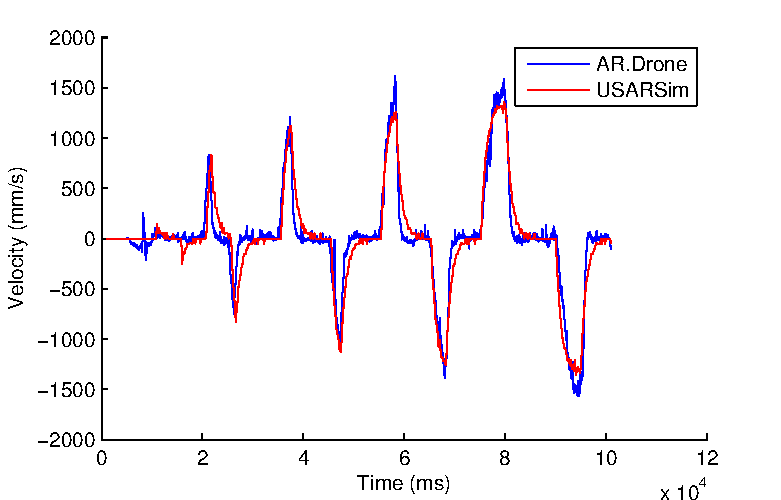
\includegraphics[width=11cm]{images/RYtdB-eps-converted-to.pdf}
\caption{Velocity of the real (blue) and simulated AR.Drone (red) on the same control pulses as shown in Figure~\ref{fig:RealResponse}.}

\label{fig:ComparisonOfResponse}
\end{figure}

As one can see, the acceleration has for the real and simulated AR.Drone nearly the same slope. The deceleration of the simulated AR.Drone is slightly lower. In the real AR.Drone the feedback loop (based on the onboard visual odometry of the ground camera) actively decelerates the system. Overall, the dynamic behavior of the simulator closely resembles the dynamic behavior of the real system. Additionally, tests with more complex maneuvers (horizontal and vertical square) have been recorded, but unfortunately not yet analyzed in detail.


\section{Position accuracy}
\label{sec:results-position-accuracy}
An experiment has been carried out to evaluate the accuracy of the AR.Drone's estimated position.
This experiment is performed above a texture-rich floor (Section \ref{sec:exp1-texture-poor}) and a texture-poor floor (Section \ref{sec:exp1-texture-poor}).
The position can be estimated using different methods and the accuracy of all these methods are evaluated.
To ensure fair comparison of the different estimation methods, a flight was recorded (Section \ref{sec:proposed-framework}) and played back to generate the same input for all methods.

The first position estimation method integrates the AR.Drone's onboard velocity (AV) measurements to estimate the position (Section \ref{sec:pose_estimation}).
Recent AR.Drone firmwares calculcate an estimated position onboard\footnote{Firmware 1.7.4}, which is used as second estimation method.
The third position estimation method uses the visual odometry method presented in this thesis (Section \ref{sec:visual-slam-visual-odemetry}).
The final estimation method uses the AR.Drone's onboard velocity (AV) for frequent position updates and the presented localization method (Section \ref{sec:localization}) to localize against the map that is constructed during flight.

The estimated position is compared against the groundtruth (real) position to calculcate the accuracy of the estimated position.
Great care was taken to collect accurate groundtruth of the AR.Drone's position.
A high-end laser range finder (LRF)\footnote{Hokuyo UTM-30LX, \url{http://www.hokuyo-aut.jp/02sensor/07scanner/utm_30lx.html}} is used to determine the position of the AR.Drone.
The LRF measures distance to objects.
A window is placed on the measurements to filter out measurements that originate from the environment.
All remaining distance measurements are assumed to originate from the AR.Drone.
The mean position of the filtered distance measurements is used as center position of the AR.Drone.
Futhermore, a white cylinder with a diameter of 9\begin{small}cm\end{small} and a height of 37\begin{small}cm\end{small} was added on top of the AR.Drone to improve its visability for the LRF.

The LRF measures the AR.Drone's position in its own reference frame.
Therefore, the AR.Drone's reference frame has to be accurately aligned with the LRF's reference frame.
This is achieved by rotating the AR.Drone before takeoff, such that it points in exactly the same direction as the LRF.
The following method was used to align the LRF and the AR.Drone (Figure \ref{fig:exp1-floorplan-align}).
First, the LRF is aligned against two poles in the environment.
The LRF is rotated until both poles obtained an equal y-distance in the LRF's reference frame.
Now, the LRF's x-axis is parallel to the poles.
Next, the AR.Drone's takeoff position and orientation are determined.
The takeoff position is marked on the floor (green star).
Another position was marked (red star) to indicate the desired heading direction of the AR.Drone.
Both marked position are parallel to the LRF's x-axis and the two poles.
Finally, a laser pointer is used to align the heading direction of the AR.Drone to the marked position.

\begin{figure}[htb]
\centering
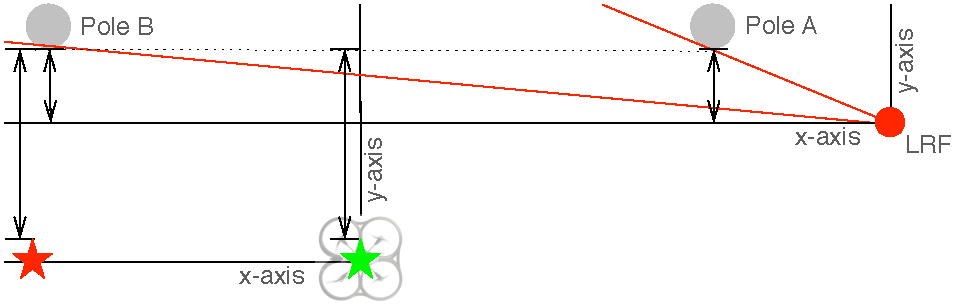
\includegraphics[width=13cm]{images/exp1-floorplan-align.pdf}
\caption{The alignment of the laser range finder and the AR.Drone. The laser range finder (LRF) is aligned against two poles. The takeoff position is marked with a green star. The red star indicates the marked heading direction of the AR.Drone. A laser pointer is used to align the heading direction of the AR.Drone to the marker position.}
\label{fig:exp1-floorplan-align}
\end{figure}








\subsection{Texture-rich floor}
\label{sec:exp1-texture-rich}
The first experiment was performed above a texture-rich floor (Figure \ref{fig:exp1-floor}), to benchmark the methods in preferable circumstances.
Magazine were spraid out on the floor to provide sufficient texture for the computer vision algorithms.
The AR.Drone flew three 8-shapes above the magazines.
An 8-shape was chosen to capture an intermediate loop.

\begin{figure}[htb!]
\centering
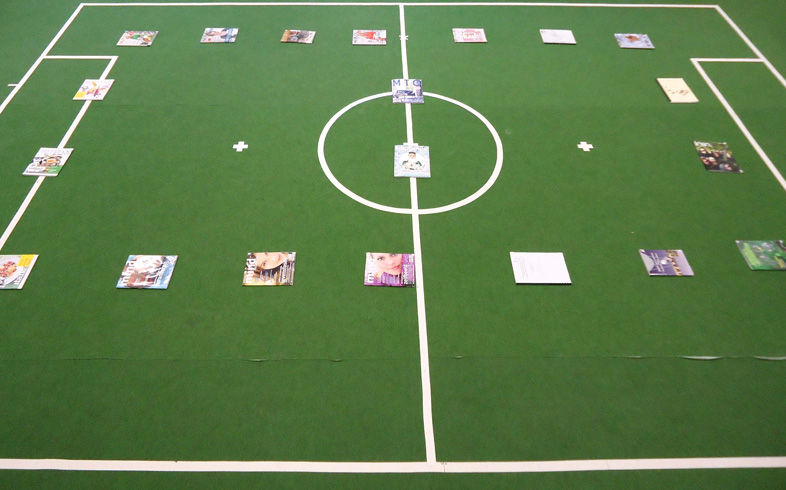
\includegraphics[width=8cm]{images/exp1-floor.jpg}
\caption{Photo of the texture-rich floor used for the first experiment. Magazine are spraid out on the floor to provide sufficient texture. The dimensions of the 8-shape are approximately $5\small{m} \times 2.5\small{m}$.}
\label{fig:exp1-floor}
\end{figure}

\begin{table}[htb!]
    \centering
    \begin{tabular}
        { | l | l | l | } 
	\hline
	Method & mean absolute error (\small{mm}) & mean relative error (percentage of trajectory length) \\
        \hline
        onboard velocity (AV) & 477 & 0.715\% \\
	onboard position (AP) & 476 & 0.714\% \\
	visual odometry (VO) & 552 & 0.828\% \\
	AV + localization & 260 & 0.390\% \\
	\hline
    \end{tabular}
    \caption{Errors made by the position estimation methods when flying above a texture-rich floor.}
    \label{tab:res_mapping}
\end{table}

The results of this experiment can be found in Table \ref{tab:res_mapping} and Figures \ref{fig:exp1-texture-error} (errors), \ref{fig:exp1-texture-path} (trajectories) and \ref{fig:exp1-texture-map} (visual map).
For the encountered circumstances, all methods are able to estimate the position quite accurately.
Both the onboard velocity (AV) method and the onboard position (AP) method produce exactly the same trajectory, which implies the onboard position estimate (AP) is based on the velocity that is estimated by the AR.Drone.

The onboard velocity (AV) slightly outperforms the visual odometry (VO) method presented in Section \ref{sec:visual-slam-visual-odemetry}.
An explanation could be that the AR.Drone features an additional optical flow algorithm that is used when the appearance-based method is performing poorly.
From Figure \ref{fig:exp1-texture-path} can be seen that the onboard velocity (AV) method has the largest error in the x-direction.
Around $54\begin{small}s\end{small}$ the error is increasing rapidly.
Analysis of the dataset pointed out that a small part of a magazine and a large part of a white line were in range of the camera.
This resulted in a velocity thas was estimated in the wrong direction along the white line, which can be recognized by the small green loop on the right side of Figure \ref{fig:exp1-texture-path}.

The visual odometry (VO) method has the largest error in the y-direction.
Around $80\begin{small}s\end{small}$ the error is increasing rapidly.
Analysis of the dataset pointed out that the magazines were out of the camera's range. During this period the velocities could not be updated.

A combination of the onboard velocity (AV) with localization against the map outperforms all other methods.
With localization against the map, the error is reduced significantly.
%The map is constructed during the first 8-shape (first $40\begin{small}s\end{small}$).
From Figure \ref{fig:exp1-texture-error} can be seen that the maximum error is not exceeding the error made during the first 8-shape.
The repetitive error pattern suggests that the error of the estimated position largely depends on the quality (accuracy) of the map, if localization can be performed regularly.
%Around $85\begin{small}s\end{small}$ the error increases rapidly. This error is caused by a false match %against the map. However, future localizations correct this mistake.

The visual map (Figure \ref{fig:exp1-texture-map}) shows that the AR.Drone's onboard white balancing is reducing the contrast of the magazines, which affects the performance of the feature detector.
This is a source of error for the visual odometry (VO) algorithm.
Futhermore, errors in the ultrasound and IMU measurements are other sources that result in errors in the estimated velocities.

% 66674 mm

\begin{figure}[htb!]
\centering
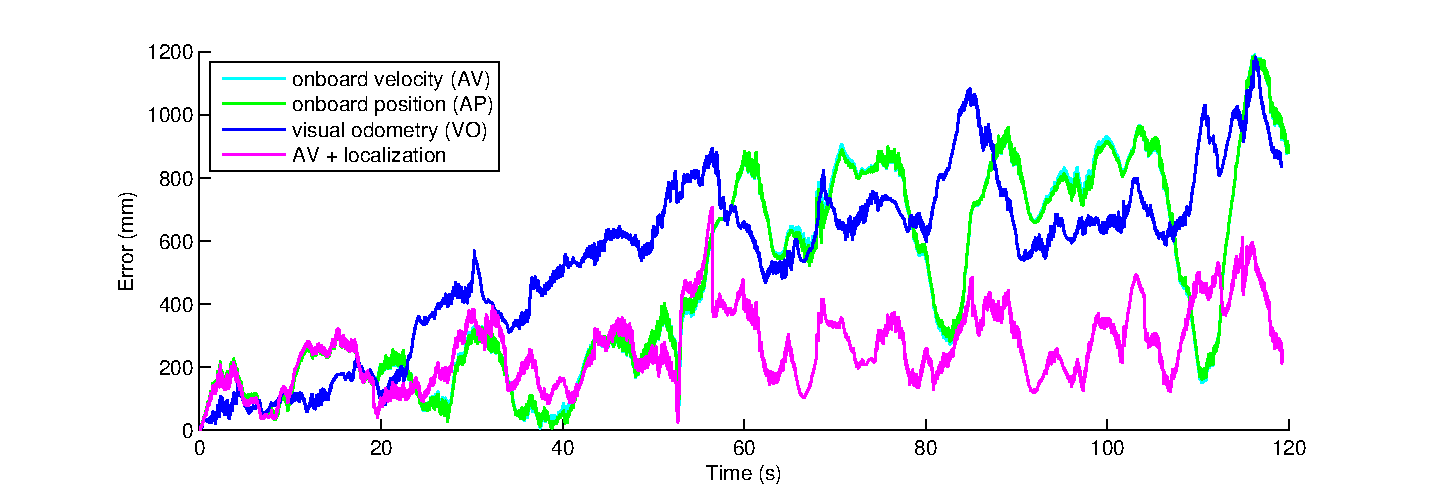
\includegraphics[width=\linewidth]{images/exp1-run13-error.eps}
\caption{Errors between the estimated positions and the groundtruth.}
\label{fig:exp1-texture-error}
\end{figure}

\begin{figure}[htb!]
\centering
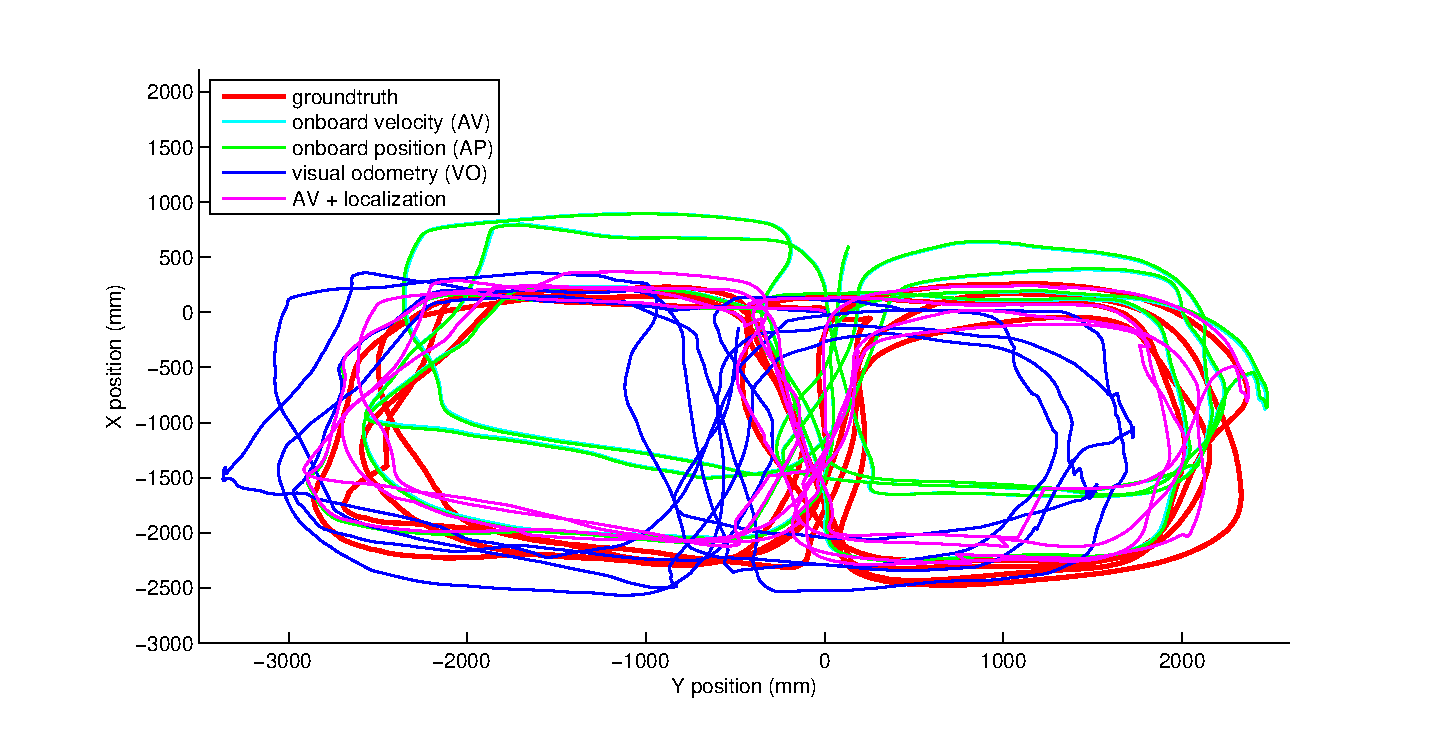
\includegraphics[width=\linewidth]{images/exp1-run13-path.eps}
\caption{Estimated trajectories of the different position estimation methods. The AR.Drone flew three 8-shapes above above a texture-rich floor.}
\label{fig:exp1-texture-path}
\end{figure}

\begin{figure}[htb!]
\centering
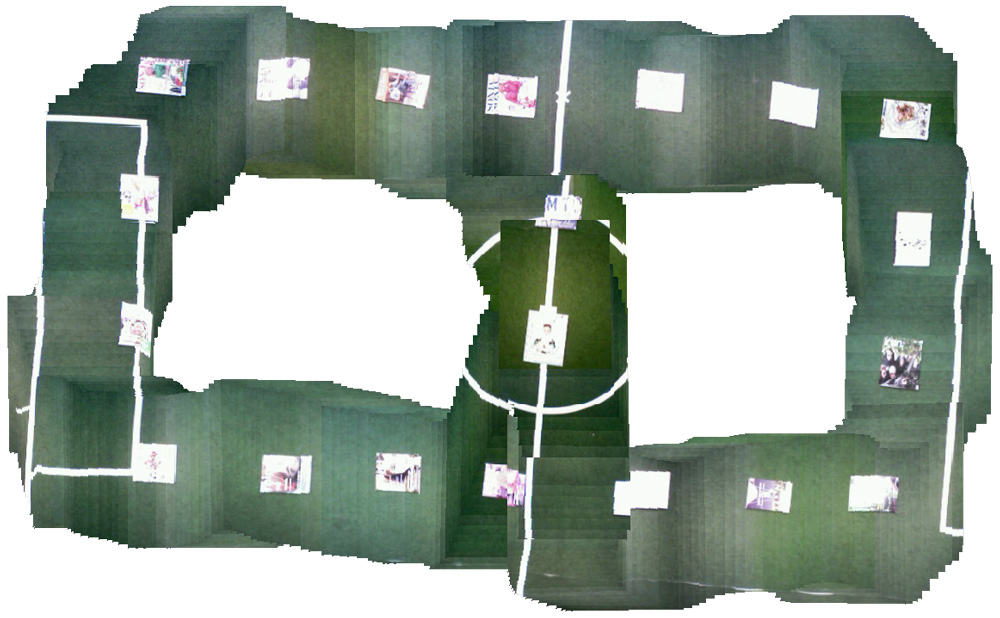
\includegraphics[width=0.75\linewidth]{images/exp1-run13-map.jpg}
\caption{Visual map created by the visual mapping method (Section \ref{sec:texture_map}). The map is constructed during the first 8-shape. The position estimates are based on the onboard velocity (AV) and the visual localization method (Section \ref{sec:localization}).}
\label{fig:exp1-texture-map}
\end{figure}




\subsection{Texture-poor floor}
\label{sec:exp1-texture-poor}
The experiment is repeated above a floor with low texture, to benchmark the methods in difficult circumstances.
Therefore, all magazines (Figure \ref{fig:exp1-floor}) are removed, resulting in a green floor with few white lines.
The AR.Drone flew a single 8-shape.


% 19616
\begin{table}[htb!]
    \centering
    \begin{tabular}
        { | l | l | l | } 
	\hline
	Method & mean absolute error (\small{mm}) & mean relative error (percentage of trajectory length) \\
        \hline
        onboard velocity (AV) & 1292 & 6.586\% \\
	onboard position (AP) & 1294 & 6.597\% \\
	visual odometry (VO) & 1126 & 5.740\% \\
	\hline
    \end{tabular}
    \caption{Errors made by the position estimation methods when flying above a texture-poor floor.}
    \label{tab:res_mapping-poor}
\end{table}


The results of this experiment can be found in Table \ref{tab:res_mapping-poor} and Figures \ref{fig:exp1-notexture-error} (errors), \ref{fig:exp1-notexture-path} (trajectories) and \ref{fig:exp1-notexture-map} (visual map).
For the encountered circumstances, all methods are unable to estimate the position accurately.
Again, both the onboard velocity (AV) method and the onboard position (AP) method produce exactly the same trajectory.
Localization was not possible and therefore omitted from the plots.

The visual odometry (VO) method slightly outperforms the onboard velocity (AV) method.
One would expect that the AR.Drone's additional optical flow method outperforms appearance-based methods.
From Figure \ref{fig:exp1-notexture-path} can be seen that the onboard velocity (AV) method fails to correctly deal with the lines on the floor.
The onboard velocity (AV) methods measures a velocity in the wrong direction along the lines, resulting in a large error.
One would expect that the onboard aerodynamic model should correct this (i.e., the angle of the AR.Drone can be used to determine the correct direction).

From Figure \ref{fig:exp1-notexture-path} can be seen that the visual odometry (VO) method underestimates the velocities.
At places where the AR.Drone changes direction, the method was able to track sufficient features (due to the presence of corners) and estimate the velocities.
At these places, the AR.Drone's velocity was below the average speed due to deaccelerations.
Along most straight parts of the trajectory insufficient features were tracked and the (higher) velocity could not be updated.
Therefore, the lower velocities during the direction changes are maintained when flying along the straight parts of the trajectory.


\begin{figure}[htb!]
\centering
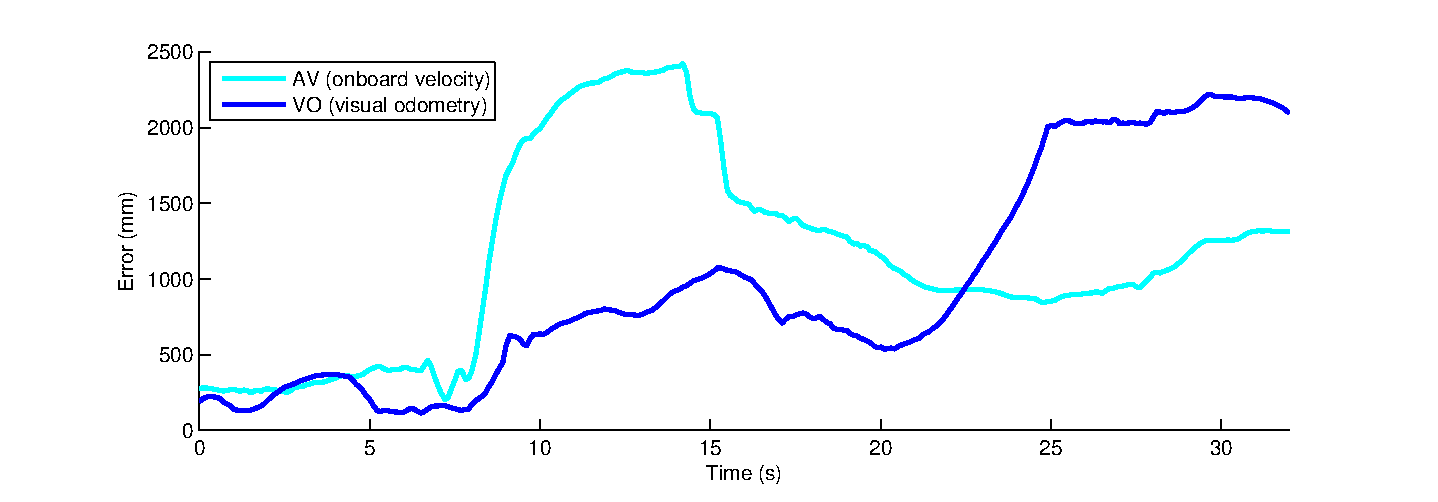
\includegraphics[width=\linewidth]{images/exp1-run2-error.eps}
\caption{Error}
\label{fig:exp1-notexture-error}
\end{figure}

\begin{figure}[htb!]
\centering
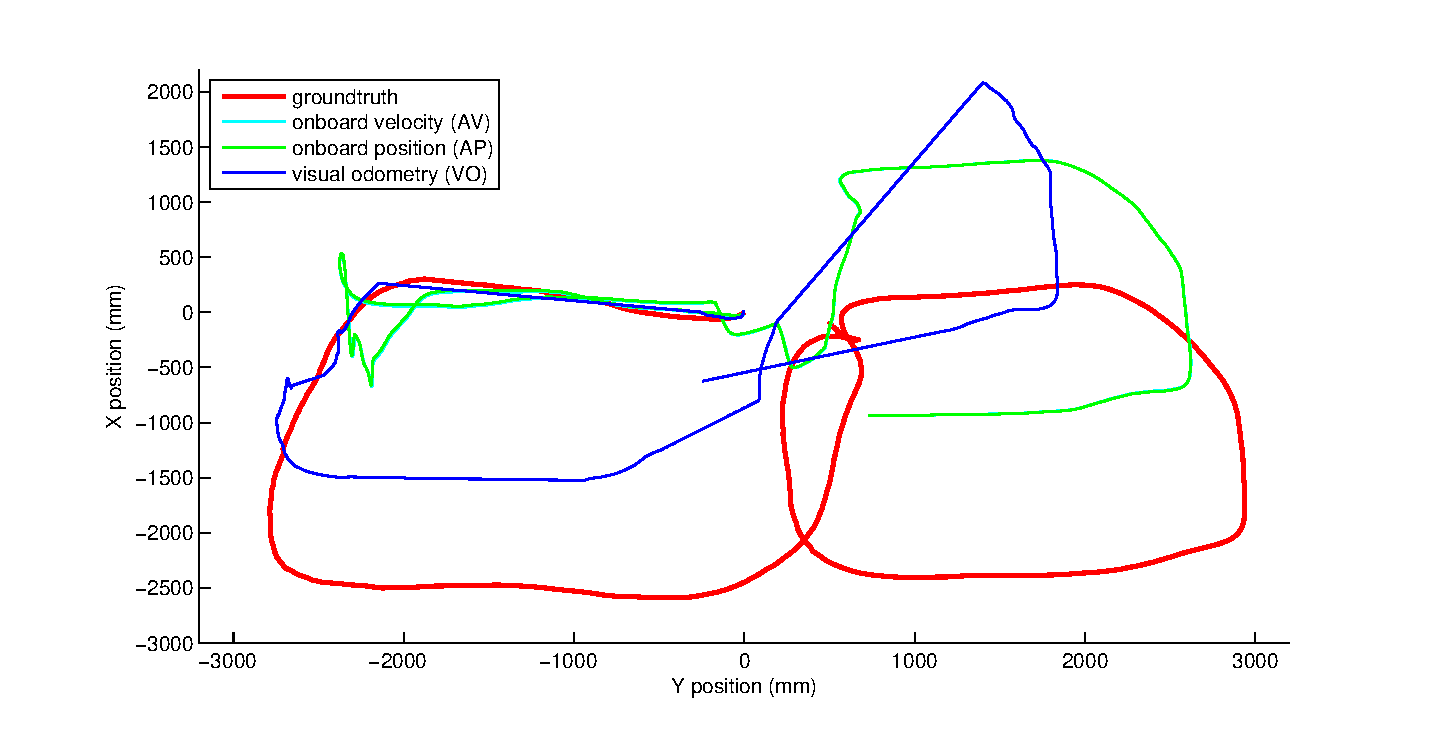
\includegraphics[width=\linewidth]{images/exp1-run2-path.eps}
\caption{Trajectory}
\label{fig:exp1-notexture-path}
\end{figure}

\begin{figure}[htb!]
\centering
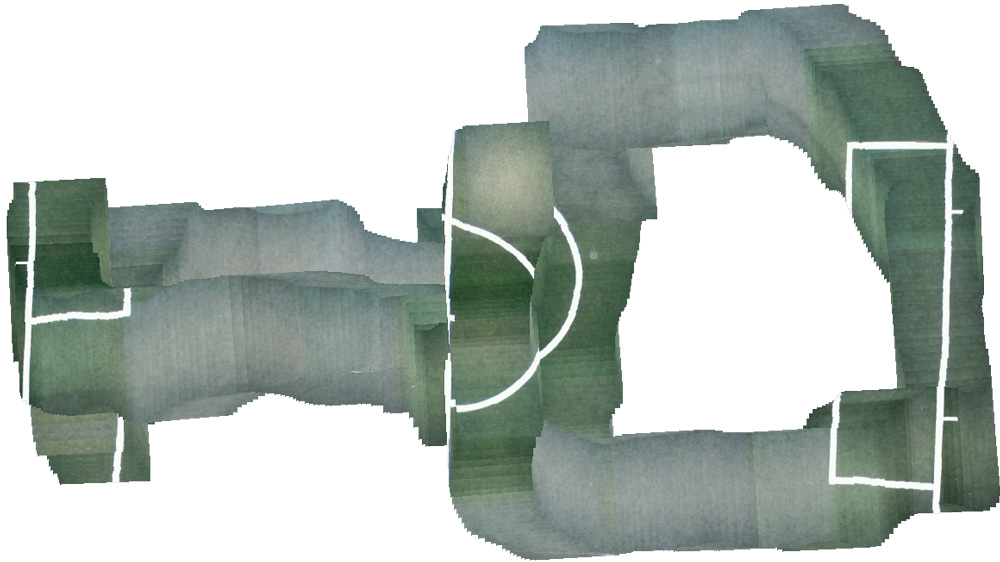
\includegraphics[width=0.75\linewidth]{images/exp1-run2-map.jpg}
\caption{Visual map created by the visual mapping method (Section \ref{sec:texture_map}). The position estimates are based on the onboard velocity (AV).}
\label{fig:exp1-notexture-map}
\end{figure}